\chapter{\textit{A Large Ion Collider Experiment}} \label{ch:alice}
In questo capitolo verrà fornita una panoramica dell'esperimento ALICE descrivendo i suoi componenti principali e le loro funzioni.
Successivamente, verrà analizzato il contributo di ALICE nella ricerca nella fisica nucleare delle alte energie, come lo studio del plasma di quark e gluoni. 
Infine, verranno introdotti i tipi di collisioni analizzate da ALICE, concentradosi sulle collisioni ione-ione, evidenziandone il ruolo cruciale per riprodurre in laboratorio le condizioni primordiali dell'universo e per investigare le proprietà fondamentali della materia.

%%%%%%%%%%%%%%%%%%%%%%%%%%%%%%%%%
\section{L'esperimento ALICE}
L'esperimento \emph{A Large Ion Collider Experiment} (ALICE) \cite{The_ALICE_Collaboration_2008} fa parte del complesso del \emph{Large Hadron Collider} (LHC), il più grande e più potente acceleratore di particelle al mondo \cite{Lyndon_Evans_2008}.
L'LHC è situato sul confine franco-svizzero nella regione di Ginevra, e si trova all'interno di un tunnel sotterraneo che raggiunge una profondità fino a 175 m.
Lungo l'anello dell'LHC sono stati realizzati quattro principali esperimenti: ALICE, CMS, LHCb e ATLAS.
Essi sono disposti secondo lo schema riportato in \autoref{fig:LHC}.
\begin{figure}[htb]
    \centering
    \includesvg[width=0.7\textwidth]{image/1-alice/LHC.svg}
    \caption{Rappresentazione schematica delle posizioni dei quattro grandi esperimenti di LHC, indicati dai punti gialli. "p" e "Pb" indicano gli acceleratori lineari dei protoni e degli ioni di Pb, PS è il \emph{Proton Synchrotron}, SPS il \emph{Super Proton Synchrotron}. (Autore: \href{https://it.m.wikipedia.org/wiki/File:LHC.svg}{Arpad Horvath}).}
    \label{fig:LHC}
\end{figure}
Il centro di ricerca responsabile dell'LHC è l'\emph{Organizzazione Europea per la Ricerca Nucleare} (CERN), fondato nel 1954 a Ginevra, in Svizzera, e fin da allora si è occupato della ricerca nel campo della fisica nucleare e subnucleare.
L'LHC non è solamente il più grande apparato sperimentale al mondo per dimensione, ma anche per numero di fisici e altri studiosi coinvolti, provenienti da qualunque angolo del mondo, rendendo il CERN senza dubbio una delle collaborazioni scientifiche più importanti del mondo.   
Tuttavia è da menzionare che l'LHC non è sempre in operatività, ma lo è solamente in alcuni periodi chiamati \emph{Run}, i quali durano anni, alternati a periodi di manutenzione e aggiornamento, chiamati \emph{Long Shutdowns} (LS).
Di \textit{Run} ad oggi ce ne sono stati tre (Run 1 2009-2013, Run 2 2015-2018, Run 3 2022-2025) e futuri \textit{Run} sono già stati programmati.
In questa tesi si considereranno i dati raccolti durante il \textit{Run} 2 di LHC.
L'LHC è capace di accelerare protoni e anche ioni pesanti (per esempio Pb) a energie ultra-relativistiche.
Questa versatilità permette lo studio delle particelle e delle loro interazioni ad energie estreme.

L'esperimento ALICE si occupa proprio dello studio della materia adronica nella fase detta Plasma di Quark e Gluoni (QGP), uno stato della materia nel quale i quark e i gluoni sono in uno stato non confinato, ottenuto con valori estremi di pressione e temperatura.
Il QGP è ritenuto essere stato la fase in cui si trovava la materia negli istanti iniziali dell'universo, prima che si formasse la materia adronica ordinaria.
Il QGP risulta essere un sistema composto da particelle che interagiscono per interazione forte, descritta dalla teoria della \emph{Quantum Chromodynamics} (QCD) del modello standard.
Perciò studiare le proprietà di questa fase rende l'esperimento ALICE insieme agli altri grandi esperimenti ad LHC, fondamentale per lo studio dei processi QCD.

In LHC, le particelle cariche vengono accelerate tramite cavità di radio-frequenza (cavità RF) che sono situate lungo la circonferenza dell'LHC e devono operare con una frequenza ben precisa in modo che le particelle possano essere accelerate correttamente.
Le particelle vengono prima accelerate da ferme al di fuori dell'LHC, formando un fascio continuo di particelle.
Successivamente, arrivati a una particolare energia (per un fascio di protoni $\sim 50$ MeV) le particelle vengono separate in pacchetti, e dopo ulteriori accelerazioni vengono immesse nell'LHC.
%%%%
%%%%%%%%%%%%%%%%%%%%%%%%%%%%%%%%%%%%%%%%%%%%%%%%%%
\section{Il rilevatore ALICE e i suoi componenti}
A seguire verrà fatta un'introduzione sulle caratteristiche di un rilevatore in generale e quali sono le grandezze principali, e in seguito sulle principali caratteristiche e componenti del rivelatore ALICE.

\subsection{Caratterizzazione di un rilevatore e le grandezze principali}
Lo scopo di un rilevatore è quello di determinare le caratteristiche della particella, come la sua identità (i.e. la sua massa), l'impulso, il suo vertice di origine, l'energia e altre caratteristiche.
Per semplificare il processo di misura si definiscono delle grandezze associabili alle particelle.
Consideriamo un generico rilevatore di forma cilindrica con al suo centro il punto di interazione (IP) e con l'asse rivolto lungo l'asse $z$.
Considerando ora una particella che viene emessa dall'IP (magari dopo uno scattering) con quadrimpulso iniziale (in \textit{}{natural units}) $p^\nu = (E,\vec p)$, con $\vec p = (p_{x}, p_{y}, p_{z})$.
Questa prosegue il suo cammino finché non interagisce con il rilevatore.
L'\emph{impulso trasverso} $p_t$ della particella è definito come 
\begin{equation}
    p_t^2 = p_x^2 + p_y^2
\end{equation}
e la sua \emph{rapidità} come 
\begin{equation}
    y = \dfrac12 \ln\left(\dfrac{E+p_z}{E-p_z}\right)
\end{equation}
Le utilità di queste grandezze è che il primo è invariante per boost lungo l'asse $z$, visto che coinvolge solamente le componenti trasversali, mentre la seconda è una misura di quanto una particella sia direzionata verso l'asse $z$.
Infatti se la particella viene emessa in una direzione giacente nel piano $xy$, si ha che $p_z=0$ perciò $y=0$.
Se invece la direzione è coincidente con l'asse $z$ si ha che $E = \pm p_z$ (supponendo un regime ultra-relativistico per cui $|\vec p| \gg m$) e quindi $y\to \pm\infty$.
Applicando un boost lungo l'asse $z$ la rapidità si trasforma seguendo la seguente espressione ($y\to y'$)
\begin{equation}
    y' = y + \dfrac12\sqrt{\dfrac{1-\beta}{1+\beta}}
\end{equation}
quindi la rapidità varia di una costante legata al boost effettuato.
Un altro vantaggio nell'utilizzare questo parametro è che la differenza di rapidità tra due particelle nel loro sistema di riferimento è uguale a quella nel sistema di riferimento del laboratorio, ossia che $y_1-y_2 = y_1'-y_2'$.

Tuttavia negli esperimenti non sempre viene utilizzato questo parametro, perché richiede la conoscenza sia di $E$ che di $p_z$.
Quindi si procede a definire la \emph{pseudorapidità}, definita come 
\begin{equation}
    \eta = -\ln\tan\dfrac\theta2
\end{equation}
con $\theta$ l'angolo di scattering, ossia l'angolo tra l'asse del cilindro e la direzione di $\vec p$.
Negli esperimenti di LHC viene usata questa variabile al posto della rapidità perché con $p\gg m$ (e quindi $E\approx p$) si ha che $y\approx \eta$, il che ne spiega l'utilizzo.
In \autoref{fig:cms} si mostra una rappresentazione schematica del sistema di coordinate utilizzato convenzionalmente nei rilevatori di LHC.

\begin{figure}[htb]
    \centering
    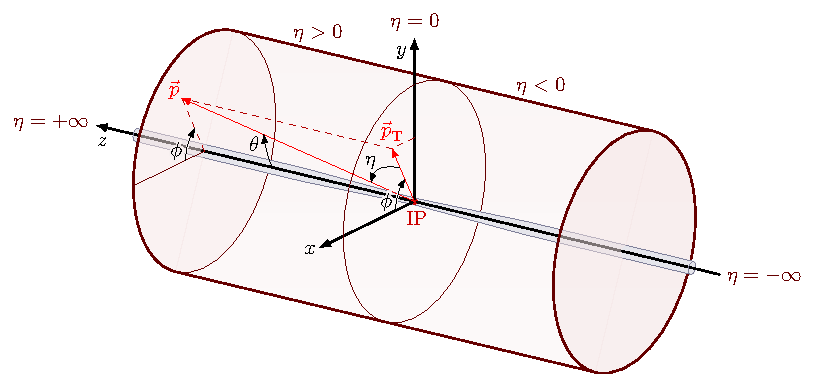
\includegraphics[width=0.9\textwidth]{image/1-alice/axis3D_CMS.pdf}
    \caption{Rappresentazione schematica del sistema di coordinate di un rilevatore in generale di LHC. "IP" è il punto di interazione, $\phi$ è l'angolo assiale, $\theta$ è l'angolo di scattering, $\eta$ è la pseudorapidità. Le particelle provengono da $-\infty$ dell'asse $z$. (Autore: \href{https://tikz.net/axis3d_cms/}{Izaak Neutelings})}
    \label{fig:cms}
\end{figure}

\subsection{Caratteristiche e principali componenti di ALICE}
Il rilevatore ALICE, ossia il complesso dei rilevatori dell'esperimento ALICE, è situato nel Punto di Interazione 2 (IP2) di LHC.
Esso è costituito da una massa di 10,000 tonnellate, lungo 26 m, alto e largo 16 m.
Occupandosi di ioni pesanti, esso deve assicurarsi di gestire bene le problematicità legate alle alte densità di particelle cariche (al tempo di design erano previste 8000 particelle cariche per unità di pseudo-rapidità, a rapidità centrali $|\eta|<1$).
Per questo motivo, per assicurarsi di ottenere delle misure di alta qualità, è necessario l'utilizzo di sensori con elevata granularità e risoluzione spaziale. 
Inoltre esso deve garantire di poter di misurare particelle che, avendo massa maggiore, verranno prodotte con l'impulso trasverso $p_t$ minore, e allo stesso modo poter effettuare la misura di particelle con $p_t$ maggiore.
Quindi, affinché ALICE possa misurare queste particelle, è necessario che il rivelatore possa ricostruire particelle in un intervallo di $p_t$ ampio, nello specifico da 100 MeV/$c$ a 100 GeV/$c$.

La struttura di ALICE è molto complessa, ma si possono individuare due parti principali:
\begin{itemize}
    \item una sezione centrale ("\emph{central barrel}") dove sono collocati i rilevatori più importanti, la maggior parte disposti geometricamente in una configurazione a guscio cilindrico.
    Questi sensori sono racchiusi da un magnete solenoidale (\emph{L3 Magnet}) che genera un campo magnetico uniforme, in direzione del suo asse, con un'intensità di $0.5$ T, necessario per la misura dell'impulso per le particelle cariche.
    In questa sezione si svolgono le mansioni più importanti di ALICE, ossia l'IDentificazione delle Particelle (PID), il tracciamento della traiettoria e la determinazione di processi che avvengono a una pseudo-rapidità di $|\eta| < 1$;
    \item una sezione esterna al magnete solenoidale per la rilevazione di muoni e comunque per misure a una pseudo-rapidità di $-4<\eta<-2.5$.
    In questa zona è presente anche un altro magnete detto \emph{magnete dipolare} con il compito di filtrare particelle indesiderate e permettere la misura dell'impulso dei muoni.
\end{itemize}
Una raffigurazione con le principali componenti di ALICE è riportata in \autoref{fig:alice}.

\begin{figure}[htb]
    \centering
    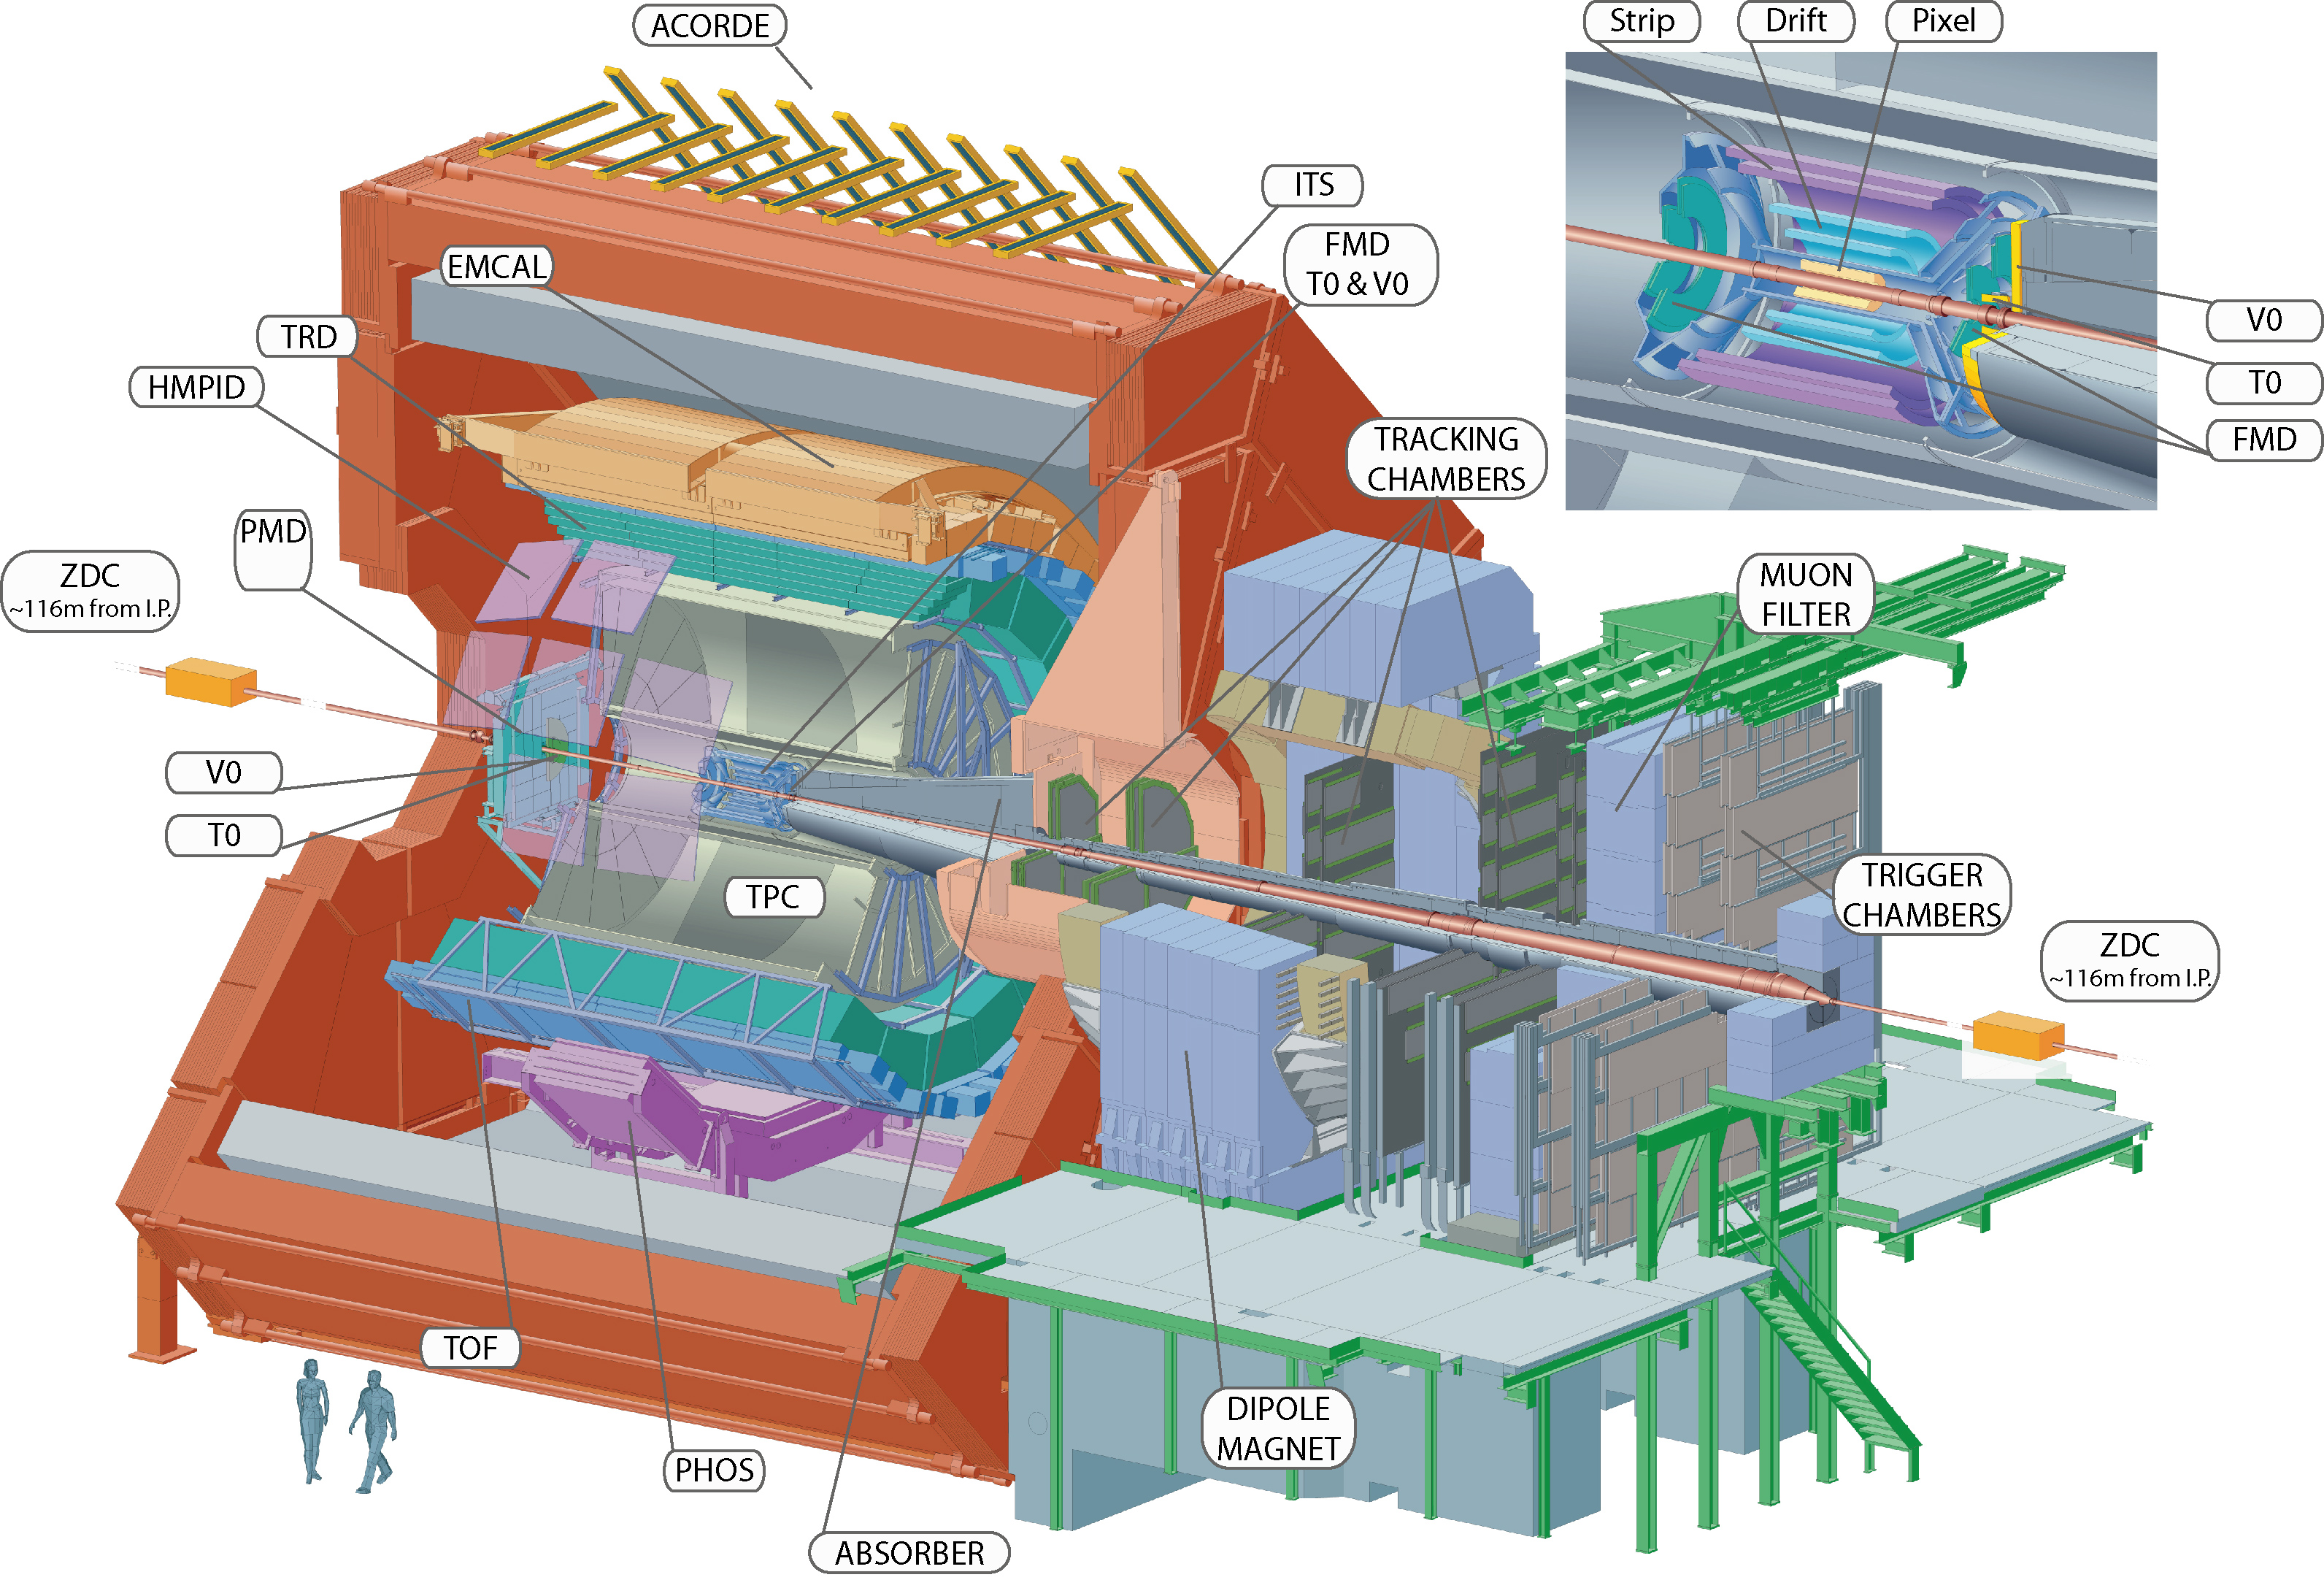
\includegraphics[width=\textwidth]{image/1-alice/alice.jpg}
    \captionwithsource{Schematica dei principali rilevatori presenti in ALICE. La struttura rossa che incapsula il \textit{central barrel} è l'\emph{L3 Magnet}.}{\href{https://en.wikipedia.org/wiki/ALICE_experiment\#/media/File:2012-Aug-02-ALICE_3D_v0_with_Text_(1)_2.jpg}{Wikimedia Commons}.}
    \label{fig:alice}
\end{figure}
Come già anticipato, nel \textit{central barrel} vi sono i rilevatori più importanti per la misura degli osservabili fisici.
Si elencano tramite una lista questi rilevatori, a partire da quello più interno a quello più esterno.

\subsubsection{L'\textit{Inner Tracking System} (ITS)}
L'\emph{Inner Tracking System}, con un diametro di appena 87 cm, ha il compito di localizzare i vertici primari delle collisioni, di ricostruire i vertici secondari, di identificazione di particelle con basso impulso trasverso ($p_t \sim 100$ MeV/$c$), tutto attraverso l'utilizzo di rilevatori al silicio, disposti in 6 piani concentrici.
L'ITS, essendo il rilevatore più interno, deve assicurarsi di raccogliere i dati con più precisione possibile perché è più vicino al luogo di interazione tra le particelle, quindi raccoglierebbe le particelle con minor vita media.
Per esempio i due stati più interni possiedono un potere risolutivo migliore di 100 \si{\micro\metre}.

\subsubsection{La \textit{Time Projection Chamber} (TPC)}
La \emph{Time Projection Chamber} è il principale rivelatore di tracciamento del \textit{central barrel}.
Essa presenta una simmetria assiale, con al centro un elettrodo ad alto voltaggio, e la superficie esterna che fa da gabbia di Faraday.
Con questa struttura le dimensioni del raggio interno ed esterno assumono il valore di $\sim 85$ cm e di $\sim 250$ cm rispettivamente.
Il compito principale della TPC è quello di misurare l'impulso di particelle cariche e di effettuare PID misurando l'energia persa per unità di distanza $dE/dx$, per particelle con $|\eta| < 0.9$.
Per la misura di questa grandezza, il volume interno è riempito con un gas (che durante \textit{Run} 2 consisteva in una miscela composta all'88\% da Ar e al 12\% da CO$_2$).
La particella perde energia per ionizzazione rilasciando  elettroni che quindi migreranno verso gli elettrodi, e il numero di elettroni rilevati sarà proporzionale alla perdita di energia della particella nel gas.

\subsubsection{Il rilevatore \textit{Time Of Flight} (TOF)}
Il rilevatore di tempo di volo \emph{Time-Of-Flight} consiste in una griglia cilindrica di rilevatori a piani resistivi multi-gap (MRPC), i quali misurano il tempo di volo delle particelle ottenendo in questo modo la loro velocità tramite la quale, insieme alla quantità di moto, è possibile ottenere la massa.
Il rilevatore ha una superficie di 141 \si{m^2} e riesce a misurare particelle con pseudo-rapidità centrale ($|\eta| < 0.9$).

\subsubsection{Il rilevatore \textit{High Momentum Particle IDentification} (HMPID)}
Il rilevatore di HMPID è dedicato all'identificazione di adroni carichi con $p_t > 1$ GeV/$c$, quindi serve come ausilio alla PID per gli altri rilevatori elencati in precedenza.
Tuttavia, questo strumento non riesce a rilevare particelle con $|\eta| >0.6$, limitando la statistica disponibile.

\subsubsection{Altri rilevatori}
Altri rilevatori sono:
\begin{itemize}
    \item Gli \emph{Zero Degree Calorimeter}, usati ad esempio per contare il numero di nucleoni spettatori, cioè che non partecipano alla collisione;
    \item Il \emph{V0 detector}, composto da due griglie circolari di scintillatori, ognuno posto sull'asse di collisione in punti opposti rispetto al punto di interazione, misurando in questo modo particelle con alta rapidità.
    Essi funzionano emettendo un segnale con intensità proporzionale al numero di particelle che li attraversano, dunque possono essere usati per la determinazione della molteplicità e della centralità a seconda della collisione considerata;
    \item Il \emph{T0 detector}, formato da due contatori Cherenkov, collocati nella stessa modalità in cui sono disposti i \textit{V0 detector}.
    Vista la disposizione spaziale, anch'essi si occupano di particelle con alta rapidità.
    Una delle loro funzioni è quella di fornire una misura precisa del tempo di collisione degli eventi, necessaria per le misure del tempo di volo.
    Esse possono essere anche utilizzate per la determinazione della posizione del vertice, tuttavia con minore precisione ($\pm 1.5$ cm).
\end{itemize}

L'identificazione di nuclei e antinuclei leggeri in ALICE viene effettuata attraverso la misura della perdita di energia specifica ($dE/dx$) e del tempo di volo delle tracce cariche effettuata da TPC e TOF, rispettivamente.
Ogni particella, infatti, assume un proprio andamento caratteristico della perdita di energia $dE/dx$ in funzione della quantità di moto.
A dimostrazione, la \autoref{fig:pid} mostra alcuni rari candidati di $^4\overline{\text{He}}$ identificati con successo nella presa dati del 2011 \cite{refId0_exotica}.
\begin{figure}[ht]
    \centering
    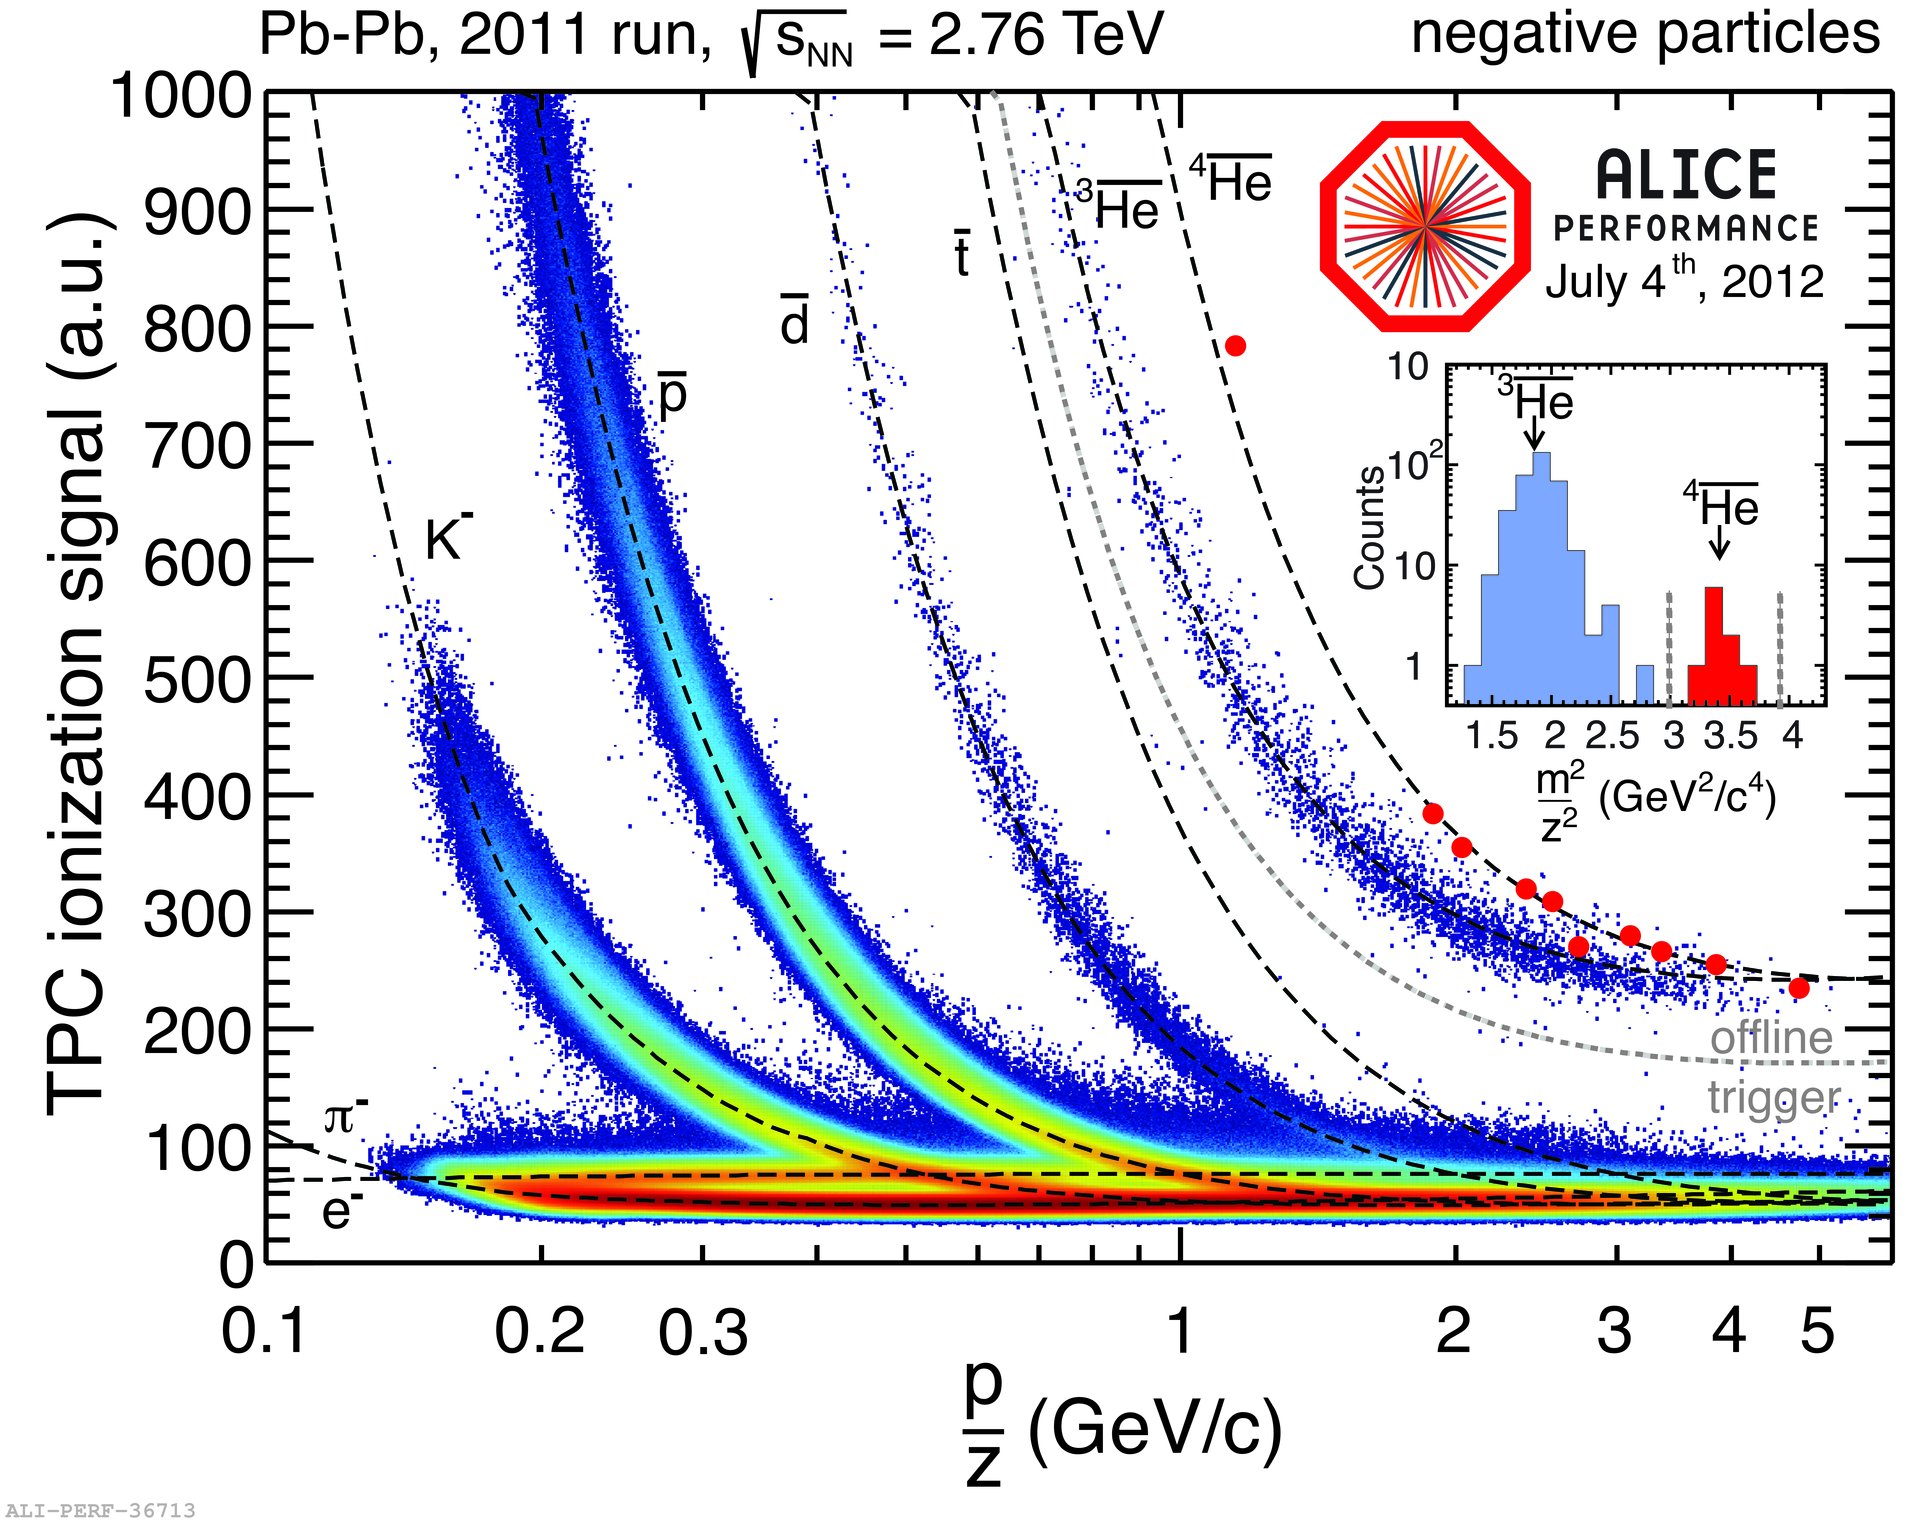
\includegraphics[width=0.7\linewidth]{image/1-alice/PID.png}
    \captionwithsource{Spettro misurato dalla TPC della perdita di energia specifica di particelle con carica negativa. Le linee tratteggiate rappresentano le previsioni teoriche, mentre i punti rossi rappresentano i candidati di $^4\overline{\text{He}}$ selezionati utilizzando la misura del tempo di volo delle anti-particelle. $\bar d$ rappresenta gli antideuteroni, $\bar t$ indica gli anti-trizi.}{\cite{refId0_exotica}}
    \label{fig:pid}
\end{figure}
%%%%%%%%%%%%%%%%%%%%%%%%%%%%%%%%%%
\section{Il ruolo dell'esperimento ALICE}\label{ch:objectives_alice}
Come già anticipato, ALICE lavora su molti punti della ricerca nel campo della fisica delle particelle.
Coinvolgendo collisioni tra particelle pesanti, ALICE gioca un ruolo fondamentale nel rispondere al quesito dell'origine dell'universo.

\subsection{Studio della formazione nucleare}
Il principale obiettivo di ALICE è quello di studiare lo stato del plasma di quark e gluoni, il quale è ritenuto essere stato lo stato della materia negli istanti iniziali dell'universo, e in particolare la transizione da questa fase alla materia ordinaria, processo chiamato adronizzazione.
Infatti ALICE, tramite LHC e le collisioni di ioni pesanti, riesce a riprodurre e analizzare questo stato della materia, caratterizzato da temperature e pressioni estreme.
Tuttavia è importante menzionare che questo stato della materia ha vita breve, dell'ordine di $\sim10^{-23}$ s (come vedremo successivamente), e si misurano solamente i prodotti di decadimento, che consistono di particelle ordinarie come protoni, neutroni e nuclei leggeri, con le corrispettive antiparticelle.
Quindi ALICE si occupa anche dei meccanismi di formazione di nuclei che non sono ancora del tutto compresi; studiare la produzione dei (anti)nuclei leggeri potrebbe fornire informazioni su questi meccanismi e permettere di testare i modelli teorici che sono stati sviluppati per descriverli.

Più dettagli saranno forniti nel prossimo capitolo.

\subsection{Materia oscura}
Si studiano gli (anti)nuclei anche per un altro scopo, ossia la ricerca di materia oscura.
Si considera la materia oscura come la componente attrattiva dominante della gravità, ma, non potendola osservare direttamente, possiamo conoscere solamente alcune proprietà di essa, attraverso misure delle velocità di rotazione delle galassie, dispersione di velocità delle galassie ellittiche, lenti gravitazionali o comunque tramite osservazioni astronomiche.
Una eventuale scoperta della materia oscura porterebbe senz'altro a una rivoluzione senza precedenti nella fisica moderna.

Ad oggi abbiamo diversi modelli per caratterizzare la natura della materia oscura, in seguito ne elenchiamo alcuni: l'ipotesi barionica della materia oscura, per cui si ipotizza la composizione barionica della materia oscura; i modelli non barionici, come il modello degli assioni, ipotetiche particelle molto leggere e caratterizzate da elevate velocità, oppure il modello dei neutrini; infine, il più promettente, il modello dei WIMP.
Quest'ultimo modello, introdotto da Steigman e Turner \cite{STEIGMAN1985375_wimp}, ipotizza l'esistenza delle particelle massive debolmente interagenti, in acronimo WIMP (\emph{Weakly Interacting Massive Particle}). 
L'abbondanza di materia oscura può essere spiegata da questo modello, in particolare dal meccanismo di \emph{freeze-out} termico, nella quale il sistema, passando dal QGP, si espande così velocemente che la velocità dell'espansione dell'universo supera la velocità di interazione delle particelle.
Perciò si possono considerare i WIMP come i relitti termici dell'universo. 
Sebbene non siano stati ancora osservati sperimentalmente, neanche indirettamente, si predice che i WIMP annichilino e decadino in (anti)materia ordinaria (per esempio antiprotoni e antineutroni), i quali possono interagire formando stati legati, ossia antinuclei leggeri.
Questi possono invece costituire un segnale rilevabile, con energia cinetica di 0.1-1 GeV alla produzione, senza problemi di eventuali fondi cosmici, dal momento in cui alcuni dei modelli di WIMP predicono un flusso massiccio di antinuclei leggeri con ordini di grandezza in più rispetto a quello del fondo, come per esempio si può vedere in \autoref{fig:he3} per il nucleo di $^3\overline{\text{He}}$.
\begin{figure}[htb]
    \centering
    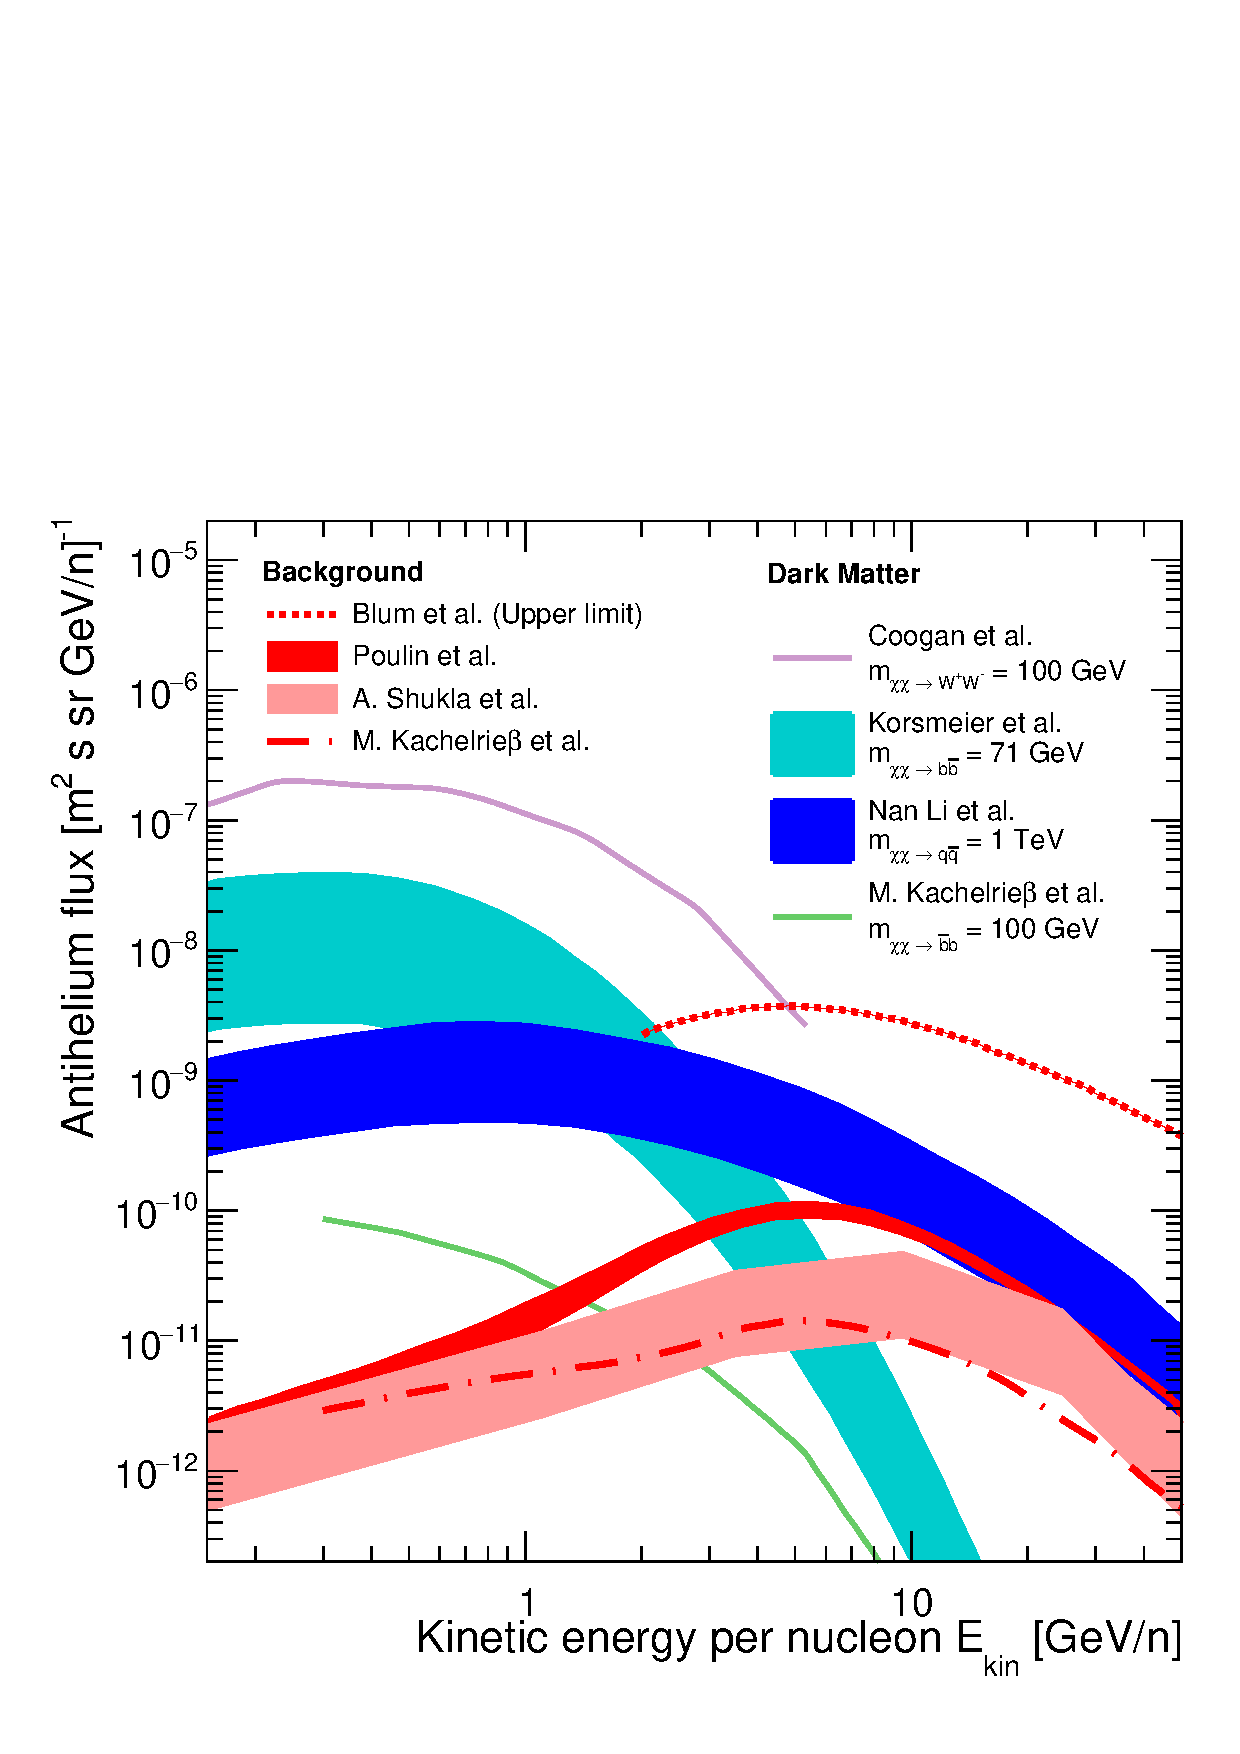
\includegraphics[width=0.6\textwidth]{image/1-alice/He3.pdf}
    \captionwithsource{Il flusso di $^3\overline{\text{He}}$ (in azzurro) in funzione dell'energia cinetica secondo più modelli di WIMP provenienti dalla letteratura scientifica, in confronto con il fondo cosmico (in rosso).}{\cite{Doetinchem_2020}.}
    \label{fig:he3}
\end{figure}

\subsection{La ricerca dei nuclei}
Per riuscire a studiare le proprietà degli (anti)nuclei è necessario come prima cosa riuscire a misurarli.
Tuttavia si noti che il numero di nuclei che viene prodotto in collisioni adroniche è molto ridotto, per cui un esperimento effettuato con un valore insufficiente dell'energia del centro di massa $\sqrt s$ comporta una percentuale molto bassa di (anti)nuclei prodotti.

Per quantificare questo numero, si considera che la formazione di un antinucleone è corrisposta necessariamente alla formazione di un nucleone, per conservazione del numero barionico.
Tenendo in considerazione ciò allora l'energia $\sqrt s$ dovrebbe assumere un valore molto più alto inizialmente.
% Per esempio per aggiungere il deuterone nel sistema è necessario l'aggiunta di 17 GeV in $\sqrt s$ \cite{2011STAREeuteronEormationEnergy}.
In generale nella letteratura si assume che venga prodotto un nucleo in ogni circa 1000 nucleoni prodotti, per nucleone del nucleo. 
Inoltre è necessario ricordare che in un evento di collisione il numero barionico deve essere conservato, per cui se l'energia iniziale è sufficientemente bassa, si vedrà uno sbilanciamento in numero, in particolare si avrà che il numero di antinuclei che vengono prodotti è più basso rispetto al numero di nuclei.
Per esempio, esperimenti condotti all'acceleratore \emph{Intersecting Storage Rings} (ISR) del CERN negli anni Settanta con collisioni pp ad energie del centro di massa di $\sqrt s \sim 50$ GeV hanno misurato un rapporto $D/\bar D$ di circa $4$ \cite{Gibson_Duane_Newman_Ogren_Henning_Jarlskog_Little_Sanford_Wu_B&Oslash;ggild_etal._2008}.

Per ovviare a questo problema è sufficiente aumentare il valore di $\sqrt s$.
Al LHC, l'energia è sufficientemente alta per poter portare il valore del rapporto di nucleo$/$antinucleo vicino a 1.
Per vedere questo, indicando con $D$ e $\bar D$ i deuteroni e gli antideuteroni rispettivamente, in \autoref{fig:ratio_of_matter/antimatter} riportiamo il grafico della frazione di $\bar p/p$ e di $\bar D/D$, dove si può osservare un avvicinamento al valore unitario con l'aumentare dell'energia.
\begin{figure}[htb]
    \centering
    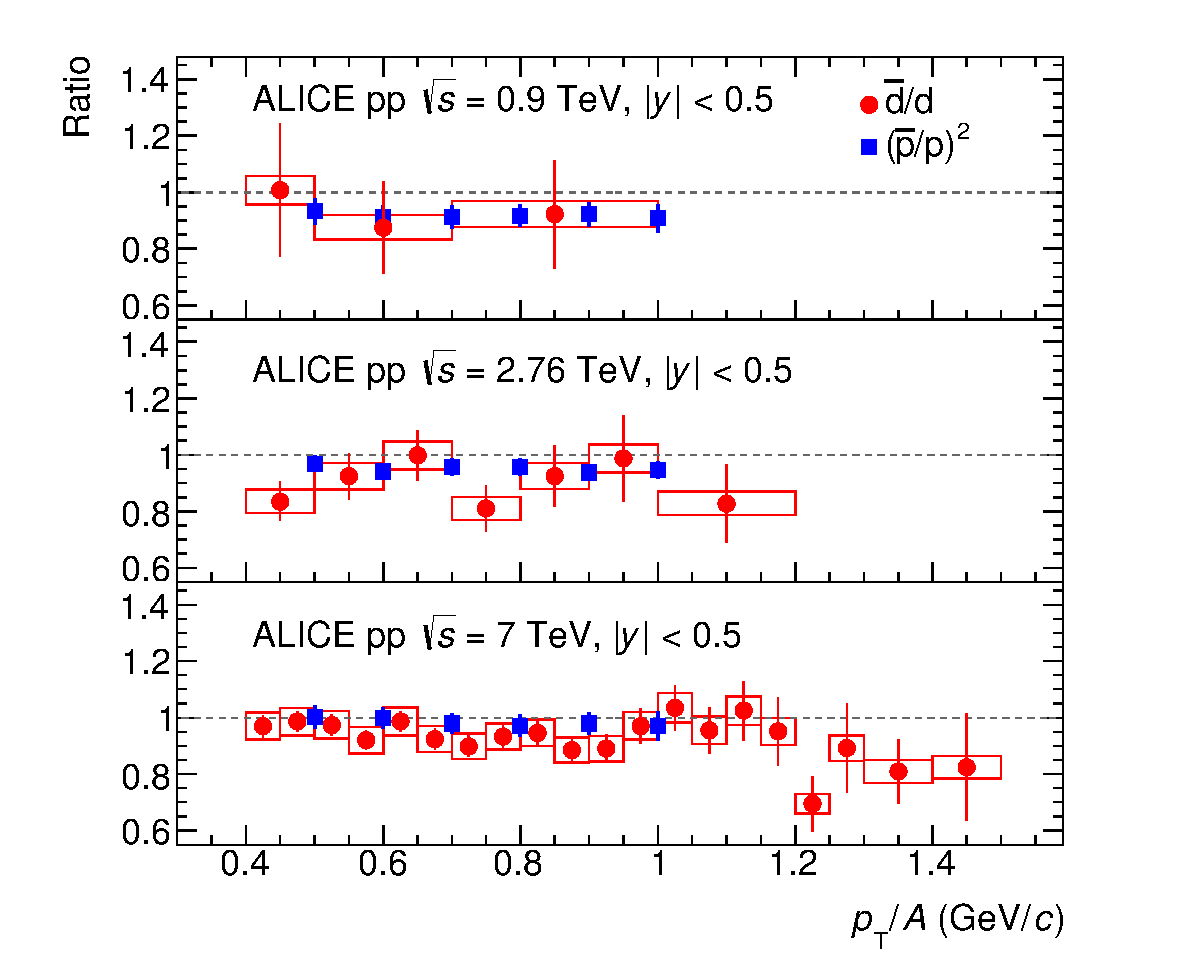
\includegraphics[width=0.7\textwidth]{image/1-alice/DbarDRatio.pdf}
    \captionwithsource{Andamento del rapporto di $\bar D/D$ (qui indicato con $\bar d/d)$ in funzione di $p_t$ per nucleone sovrapposta al rapporto quadro di $\bar p/p$, ai tre valori di energia indicati.}{\cite{Acharya_2018}.}
    \label{fig:ratio_of_matter/antimatter}
\end{figure}

\section{Collisioni in ALICE}
In questa sezione si cerca di introdurre la fisica delle collisioni riguardanti le collisioni ultrarelativistiche di ioni.

Nel Modello Standard si descrivono tre delle quattro forze fondamentali: la forza forte, la forza elettromagnetica, la forza debole in ordine di intensità.
Dalla teoria della cromodinamica quantistica (QCD) si sa che ogni nucleone è composto da quark, i quali interagiscono tramite l'interazione forte attraverso lo scambio di gluoni.
Dalla QCD inoltre sappiamo che il gluone in realtà non è altro che un quanto di energia dei campi mediatori della forza forte, e tramite un'invarianza di gauge locale SU(3) si ricavano 8 tipi di gluoni, tutti con carica di colore diversa in modo da formare una base per coprire tutti i colori possibili.\\

\subsection{Il sistema pre-collisione}
Per ricreare le condizioni richieste per la formazione di QGP è possibile far collidere ioni pesanti a regime ultra-relativistico.
In questo regime, con la contrazione di Lorentz lungo la direzione del fascio, gli ioni appaiono come dei dischi piatti (\autoref{fig:pb}), e per questo motivo le dimensioni trasversali del nucleo appaiono più larghe delle dimensioni longitudinali. 
Perciò una collisione tra ioni può essere considerata come la sovrapposizione di collisioni individuali tra i nucleoni provenienti da direzioni opposte.
\begin{figure}[htb]
    \centering
    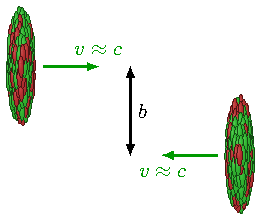
\includegraphics[width=0.5\textwidth]{image/1-alice/PbPb_collisions.pdf}
    \caption{Schema rappresentativo di una collisione Pb-Pb. Le sfere rosse rappresentano i protoni e le sfere verdi i neutroni. (Autore: \href{https://tikz.net/pbpb_collisions/}{Izaak Neutelings})}
    \label{fig:pb}
\end{figure}

È importante notare che non sempre tutti i nucleoni partecipano alla collisione: questo succede se nel piano del fascio i baricentri dei nuclei non non coincidono ma sono separati da una distanza $b$ (parametro di impatto), in questo caso interagiranno soltanto i nucleoni all'interno dell'area di sovrapposizione nucleare. 
I nucleoni non interagenti sono chiamati \emph{spettatori}; i nucleoni che viceversa partecipano alla collisione vengono chiamati \emph{partecipanti}.
Se il numero di nucleoni partecipanti è $N_\text{part}$, il numero di spettatori è $N_\text{spect} = 2A-N_\text{part}$.
Il parametro d'impatto $b$ gioca un ruolo fondamentale nelle collisioni di nuclei: esso determina la centralità di una collisione, una quantificazione della regione di sovrapposizione, e con ciò il numero di nucleoni partecipanti.
%Da questo si può capire che, se si vuole più statistica, è necessario minimizzare questo parametro massimizzando così la centralità della collisione.
Dal momento che la centralità è correlata con la molteplicità di una collisione, ossia il numero di particelle cariche prodotte nella collisione, affinché si possa normalizzare le osservabili tra collisioni differenti, la misura della centralità è fondamentale.

Vi sono due metodi principali per la misura della centralità:
\begin{itemize}
    \item Il primo metodo consiste nella misura diretta della molteplicità, tramite conteggio del numero di particelle cariche prodotte in una collisione.
    Questo metodo è tuttavia dipendente dalla scelta del modello geometrico utilizzato per i processi adronici;
    \item il secondo metodo invece si basa sulla misura dell'energia degli spettatori, in genere effettuata in posizioni di alta molteplicità.
    Questo modello, al contrario del primo, è indipendente dal modello di collisione utilizzato.
\end{itemize}

\subsection{Il sistema post-collisione}
Grazie all'alta densità di energia che si viene a creare nell'urto ultra-relativistico tra ioni pesanti, si viene a formare un sistema che interagisce per l'interazione forte, il QGP.
Lo studio di questo sistema è proprio l'obiettivo di ALICE, ossia quello di andare a indagare lo stato del QGP.
In questo stato l'energia del sistema rende l'interazione forte meno dominante, portando a uno stato deconfinato di materia in cui i quark e i gluoni possono muoversi liberamente.
\begin{figure}[htb]
    \centering
    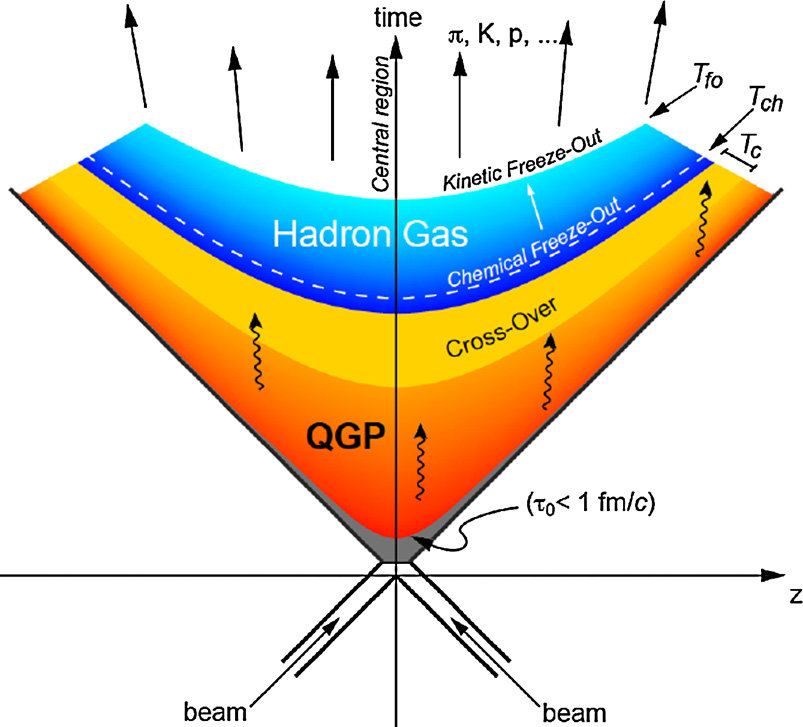
\includegraphics[width=0.7\textwidth]{image/1-alice/Colour-online-Space-time-diagram-of-a-heavy-ion-collision-of-two-nuclei-colliding-at.jpg}
    \captionwithsource{Diagramma spazio-tempo di una collisione di due ioni pesanti ultra-relativistici. La zona grigia sottostante alla QGP rappresenta lo stato di pre-equilibro.}{\cite{QGPbraun}}
    \label{fig:qgp}
\end{figure}

Più precisamente, al momento dell'impatto degli ioni, le singole collisioni coinvolgono scattering "hard" ovvero con un alto trasferimento di impulso che inducono alla produzione di partoni ad alta energia.
In questo momento si distinguono due zone in particolare: la prima a rapidità centrale, dove si è depositata la maggior parte dell'energia, la seconda invece ad alta rapidità, popolata da quark di valenza e particelle spettatori.
Nella zona a rapidità centrale, se la densità di energia è sufficientemente alta, si forma il QGP, sotto forma di \emph{fireball} in equilibrio termico.
In questa fase di equilibrio la \textit{fireball} si espande per via della pressione esercitata alla sua superficie e di conseguenza si ha un calo progressivo della temperatura; una volta che la temperatura sarà scesa al di sotto del valore critico inizia il processo di adronizzazione.
Successivamente, non appena lo scambio di impulso diventa insufficiente per sostenere le interazioni inelastiche, allora si arriva al cosiddetto \emph{freeze-out chimico}, in cui le abbondanze relative delle particelle rimangono invariate.
Nel momento in cui le particelle prodotte non interagiscono più, conservando il loro quadrimpulso, allora si parla di \emph{freeze-out cinetico}.
Infine, dopo $\sim15$ fm/$c = 5\cdot 10^{-23}$ s gli adroni formatisi giungono ai rilevatori.
Uno schema spazio-tempo di quanto appena descritto è rappresentato in \autoref{fig:qgp}.